\documentclass[journal=jprobs,manuscript=article]{achemso}

\usepackage[version=3]{mhchem} % Formula subscripts using \ce{}
\usepackage[T1]{fontenc}       % Use modern font encodings
\usepackage{multirow}
\usepackage{subcaption}

\newcommand*\mycommand[1]{\texttt{\emph{#1}}}

\author{Stefan K. Solntsev}
\email{solntsev@wisc.edu}
\author{Michael R. Shortreed}
\author{Brian L. Frey}
\author{Lloyd M. Smith}
\affiliation[UwMadison]
{University of Wisconsin-Madison}

\title[Rapid and Accurate Global PTM Discovery (G-PTM-D) Using Post-Acquisition Spectral Calibration and Defined Mass Windows]
  {Rapid and Accurate Global PTM Discovery (G-PTM-D) Using Post-Acquisition Spectral Calibration and Defined Mass Windows}

\begin{document}

\begin{abstract}

Correct identification of protein posttranslational-modifications (PTMs) is crucial to understanding many aspects of protein function in biological processes.
G-PTM-D\cite{Li_2016} is a recently developed tool for global identification and localization of PTMs.
Spectral file calibration prior to applying the tool, and algorithmic improvements in the peptide database search greatly improve the accuracy and efficiency of PTM identification.
We enhanced G-PTM-D by using targeted mass-window searches, and demonstrate its effectiveness in identification of numerous types of PTMs, including high-mass modifications such as glycosylations.
The proposed changes lead to a 20\% increase in the number of identified modifications and an order of magnitude decrease in the search time.
Targeted mass-windows searches are also shown to be useful as a replacement to a standard wide-mass search, resulting in a 10\% increase in the number of confidently identified peptides: this leads to improvements in novel modification discovery heuristics originally based on the wide-mass search.
\end{abstract}

\section{Introduction}

Many peptide residue modification types are known, and databases containing detailed information about such modifications are readily available.
Information about a modification can include the chemical or isotopic composition, mass, specificity to certain residues, and possible restriction of placement to peptide or protein termini.
While this data is almost comprehensive, information about the localization of these modification to certain residues in specific proteins is scarce.

Numerous procedures for identification and localization of PTMs from "bottom-up" tandem mass spectrometric datasets exist, e.g. MODa\cite{Na_2011}.
G-PTM-D\cite{Li_2016}, a recently described bioinformatics tool for the discovery and localization of new PTMs, is the foundation for the work described in this paper.
The G-PTM-D workflow consists of three stages: 1) A wide-mass database search\cite{Chick_2015, Na_2011} that provides spectral matches to unmodified peptides along with the mass differences between the identified peptides and the measured parent peptide masses (hypothesized to differ in mass due to the presence of a PTM).
2) For those peptides for which the mass difference corresponds to the mass of a known PTM, a database augmentation step adds plausible localized PTMs to the proteins in the search database.
3) A final standard narrow-mass search of the augmented database to identify both modified and unmodified peptides subject to the standard FDR threshold (e.g. 1\% FDR).

As described, G-PTM-D has a few significant limitations.
The initial wide-mass search procedure is slow, taking hours for modest size datasets.
Due to this, high mass modifications, such as glycosolations are out of reach, since widening the search window from the suggested $\pm 200$ Daltons increases the search time even more.
Furthermore, in G-PTM-D, modification discovery is limited to PTMs in the Uniprot database. 
Finally, PTMs that are similar in mass, such as Phosphorylation and Sulfonation are problematic since they are virtually indistinguishable in unprocessed spectra files. 

Spectral calibration prior to running the G-PTM-D procedure is essential for distinguishing modifications with similar mass.
As a side effect, calibration signinficantly increases the overall number of confidently identified peptides and modifications.

We propose an enhancement to G-PTM-D, that addresses the long search times of the wide-mass search, and the limitations of the standard final narrow-mass search.
The wide-mass search is replaced by a notch search in the discovery phase, using notches centered at the monoisotopic mass differences introduced by known modifications.
This change improves the specificity and significantly decreases search time.
The final narrow-mass search is also replaced by a notch search, further increasing the number of confidently identified peptides.

The idea of restricting the search space by only allowing certain mass differences between the precursor and the identified peptide mass is useful in other procedures as well, beyond the G-PTM-D workflow.
Its efficacy is demonstrated in context of a search for novel modifications, which is usually based on a wide-mass or an open-mass search.
A combination of specialized notch and interval searches produces superior identification and discovery results.

\begin{figure}
  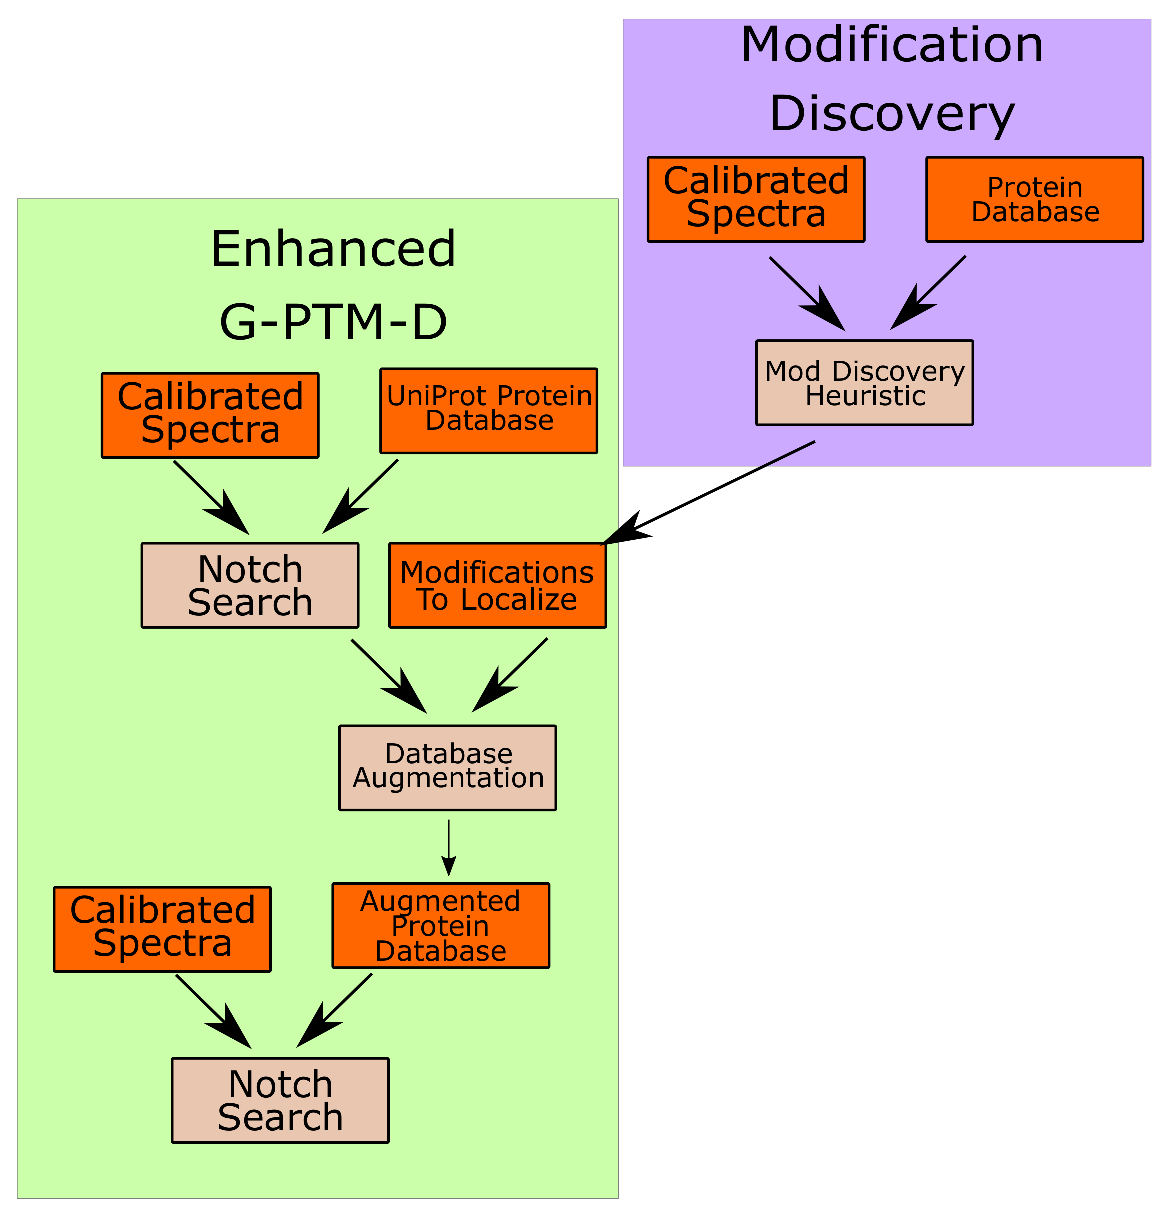
\includegraphics[scale=0.5]{diagram.eps}
  \caption{Workflows}
  \label{fgr:diagram}
\end{figure}


\section{Experimental Procedures}
We developed a modified version of the Morpheus software for bottom-up spectral database searching\cite{Wenger_2013} that we call MetaMorpheus, which integrates the database search procedure with spectral calibration and the Enhanced G-PTM-D workflow.
Two multi-fraction mammalian datasets (\textit{Mouse} and \textit{Jurkat}) with deep proteome coverage were used to evaluate the performance of the methods: these datasets are described in detail in~\cite{Shortreed_2015, Cesnik_2016}.
Uniprot XML protein databases acquired on Feb 27, 2017 containing only reviewed human/mouse proteins were employed. 

A 10ppm precursor mass tolerance was used for the initial calibration step, and then reduced to 5ppm for subsequent notch searches.
For the database augmentation step, we allowed 120 modifications including PTMs, adducts, and chemical modifications.
Final notch search used notches centered at \{0, 1.003, 2.005, 3.008\} in order to capture missed identifications due to missed monoisotopic peaks.

For the discovery of novel modifications, we used a combination of two searches: A notch search with notches at all combinations of up to 2 residue mass additions or removals, and an interval search with lower bound of -187 Daltons, and with exclusions at masses corresponding to the notch search.

\section{Results and Discussion}

Post-acquisition calibration is a useful tool that is shown to increase the number of confidently identified peptides, and enables qualitatively distinguishing modifications with similar mass.
Then, mass-window searches are contrasted with narrow-mass and open-mass searches.
The improvements in the performance of the enhanced G-PTM-D over the originally proposed G-PTM-D, that are due to using mass-window searches are shown.
Finally, the application of mass-window searches to the discovery of novel modifications is discussed.

\subsection{Calibration}

A critical parameter for peptide identification and PTM localization is mass accuracy\cite{Scherl_2008}.
Higher mass accuracy provides increased specificity and thus confidence in peptide identifications, decreasing the false discovery rate.
Instrument noise, systemic drift and miscalibration limit the mass accuracy in acquired spectra.
Multiple calibration strategies to improve mass accuracy have been devised, and fall into three general categories:  External calibration prior to the MS experiment (e.g. standard instrument calibration protocols); internal calibration during the MS experiment (e.g. real-time calibration using a lock mass standard\cite{Olsen_2005}); and subsequent to the MS experiment (post-acquisition spectral calibration, REF).
We use a post-acquisition calibration procedure, that builds upon the software lock mass concept\cite{Cox_2011} recently reported by the Mann group.
In our strategy, the m/z differences between expected and observed peaks in the peptide tandem ms spectra are compiled, and then used to recalibrate the spectra.
The increased mass accuracy of the recalibrated spectra leads directly to improved identifications of both modified and unmodified peptides, as well as to increased confidence for PTM localization.

The spectral calibration procedure consists of two steps: Step 1: A standard tolerance (e.g. 10 ppm) database search is performed on the dataset.
This yields a set of peptide identifications subject to a desired false discovery rate (e.g 1\%; based upon the target:decoy strategy (ref)).
Step 2:  The identifications from step 1 are used to extract peak matches from the spectra, and a calibration procedure is performed.
The calibration algorithm is described in detail in Supplementary Material 1.
A simple test of the calibration quality is to withhold some known peak matches from the inputs of the calibration software, and to determine if they have been shifted closer to the theoretically correct value.
We withheld 30\% of identifications, and measured the standard deviation and the average errors of the peak differences for the monoisotopic MS1 peaks with known charge states.
The average mass error went down from -3.67ppm to -0.15ppm in the jurkat dataset and from -3.32ppm for the mouse dataset.
The standard deviations decreased from 3.64ppm to 2.82ppm, and from 3.07ppm to 2.54ppm for the jurkat and mouse datasets respectively.
Figure 2 shows the clear improvement in the error for the withheld identified peptides, as a result of applying spectral calibration.

A 10 ppm narrow tolerance search produces matches with mass differences in ppm given in~\ref{fgr:figure1}.
The average and standard deviations along with 1, 2, and 3 standard deviation widths are given in Table~\ref{tbl:calib}.

\begin{table}
  \caption{Calibration Results: ppm Mass Differences}
  \label{tbl:calib}
  \begin{tabular}{llll}
    \hline
    & prior& after smooth & after rf  \\
    \hline
    stdev&	1.553	&1.039&	0.898 \\
	avg&	-3.148&	0.204&0.215\\
	68.3\% within	& [-4.701,-1.595 ]&	[-0.834,1.243	]&	[-0.683,1.114]\\
	95.4\% within&[	-6.254,	-0.042]&[	-1.873,2.282]&[	-1.581,	2.012]\\
	99.7\% within&	[-7.807,	1.511]&[	-2.912,3.321]&[	-2.479,	2.910]\\
    \hline
  \end{tabular}
\end{table}


\begin{figure}
  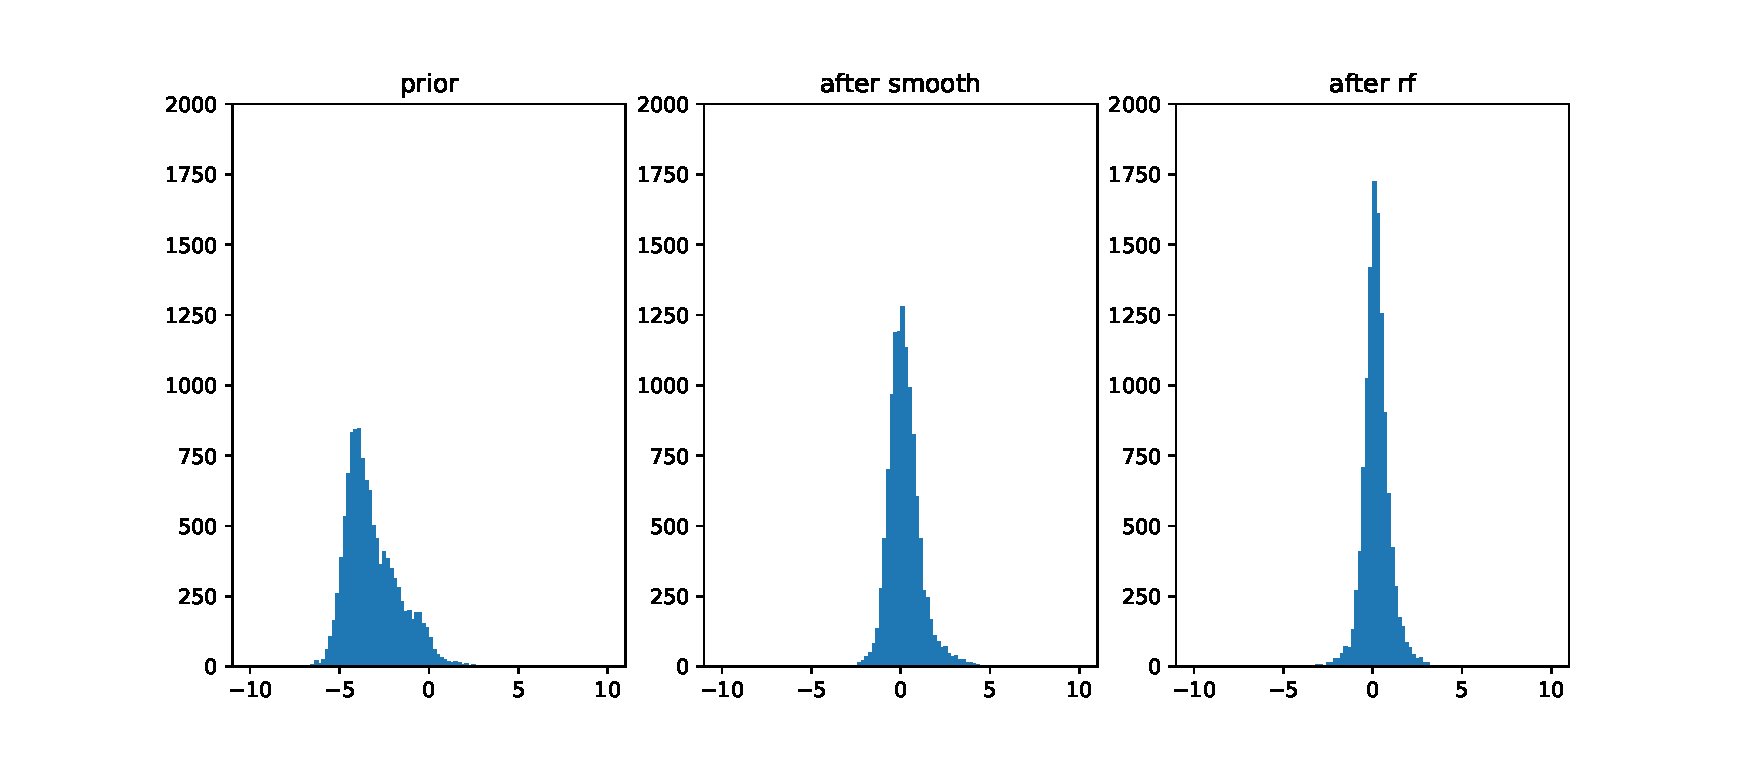
\includegraphics[scale=0.6]{figure_1.eps}
  \caption{An example figure}
  \label{fgr:figure1}
\end{figure}

\subsection{Mass-Window Searches}


A standard \textit{narrow-mass} search considers matching theoretical peptides to spectra if the peptide mass and the identified precursor mass are equal, within some tolerance (i.e. 5ppm, or 2.1 Da).
A \textit{wide-mass} search matches peptide fragment masses to fragmentation spectra while allowing large differences (i.e. $\pm 500$ Da) between the observed precursor mass and the peptide mass.
An even less restrictive \textit{open-mass} search, matches peptides from a database to fragmentation spectra without taking the precursor mass into account.
We propose alternatives to these search modes, namely a \textit{notch search} and an \textit{interval search} that fall under a broad category of \textit{mass-window} searches.
The notch search is an extension of the narrow-mass search: it allows exact matches (within a tolerance) to specific mass differences between the theoretical peptide and observed precursor masses.
The interval search is an extension of the wide-mass search: specific problematic mass differences are excluded from allowed matches.
The smaller the fraction of the mass space, and the narrower the mass window per search element, the faster the search will run (as fewer searches are executed per mass spectrum).
Figure~\ref{fgr:differentSearchModes} provides a convenient way to visualize the various search modes.

\begin{figure}
  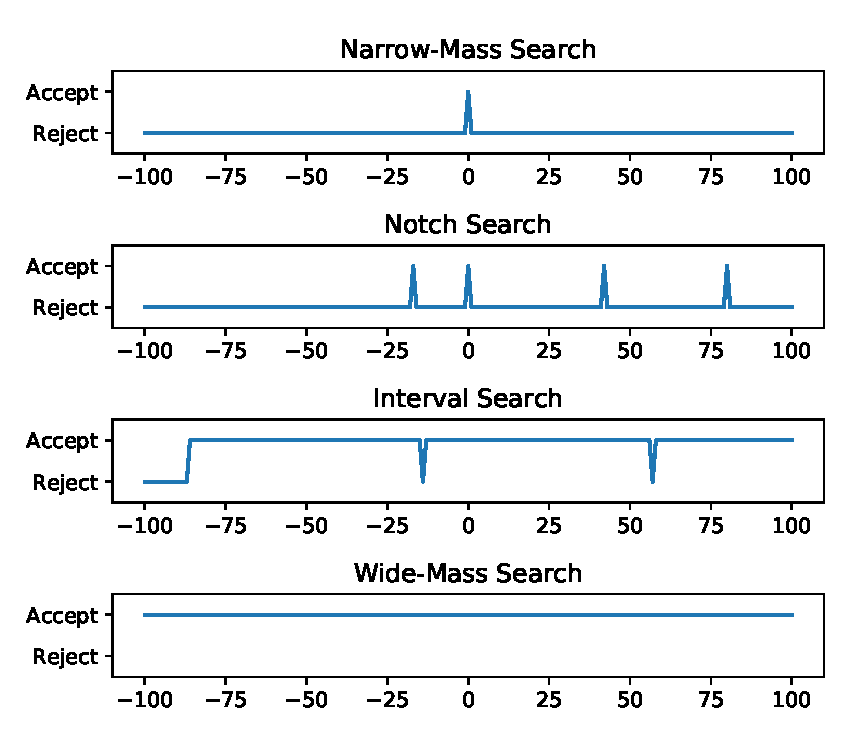
\includegraphics{figureDifferentSearchModes.eps}
  \caption{Search Modes}
  \label{fgr:differentSearchModes}
\end{figure}

\subsubsection{Notch Search vs Narrow-Mass Search}

The purpose of a narrow-mass search is to use the provided precursor mass along with fragmentation spectra information to find an exact match in a protein database.

One has to be extremely careful in using a narrow-mass search beyond a nominal tolerance of 5 or 10 ppm. 
While it does provide more identifications, a search within say $\pm 3.1$ Daltons should be done with great care.
We only recommend such a search after peaks that correspond to modifications/sequence differences are excluded.

\subsubsection{Mass Window Searches vs Open-Mass Search}

Restricting the allowed precursor masses is beneficial in searches that are intended to discover mass shift peaks.
We ran a completely open precursor mass search, and restricted ourselves to looking at 1\% FDR matches, both targets and decoys.
The plots in Figure~\ref{fig:figure2-upperlowerbounds} show the FDR in the list filtered by using a lower or upper bound cutoff on the allowed mass shifts.
It shows the fundamental difference between upper and lower bound cutoffs: while it is beneficial to restrict open searches to ignore large negative values, restricting matches with a large positive mass difference has a negative effect on the overall FDR.

This effect can be explained by the fact that it's easier to match long sequences to short peptide fragmentation profiles than it is to match short sequences to fragmentation pattern of a long peptide.

\begin{figure}
\caption{Upper and Lower bound cutoffs in Mouse Data}
\label{fig:figure2-upperlowerbounds}
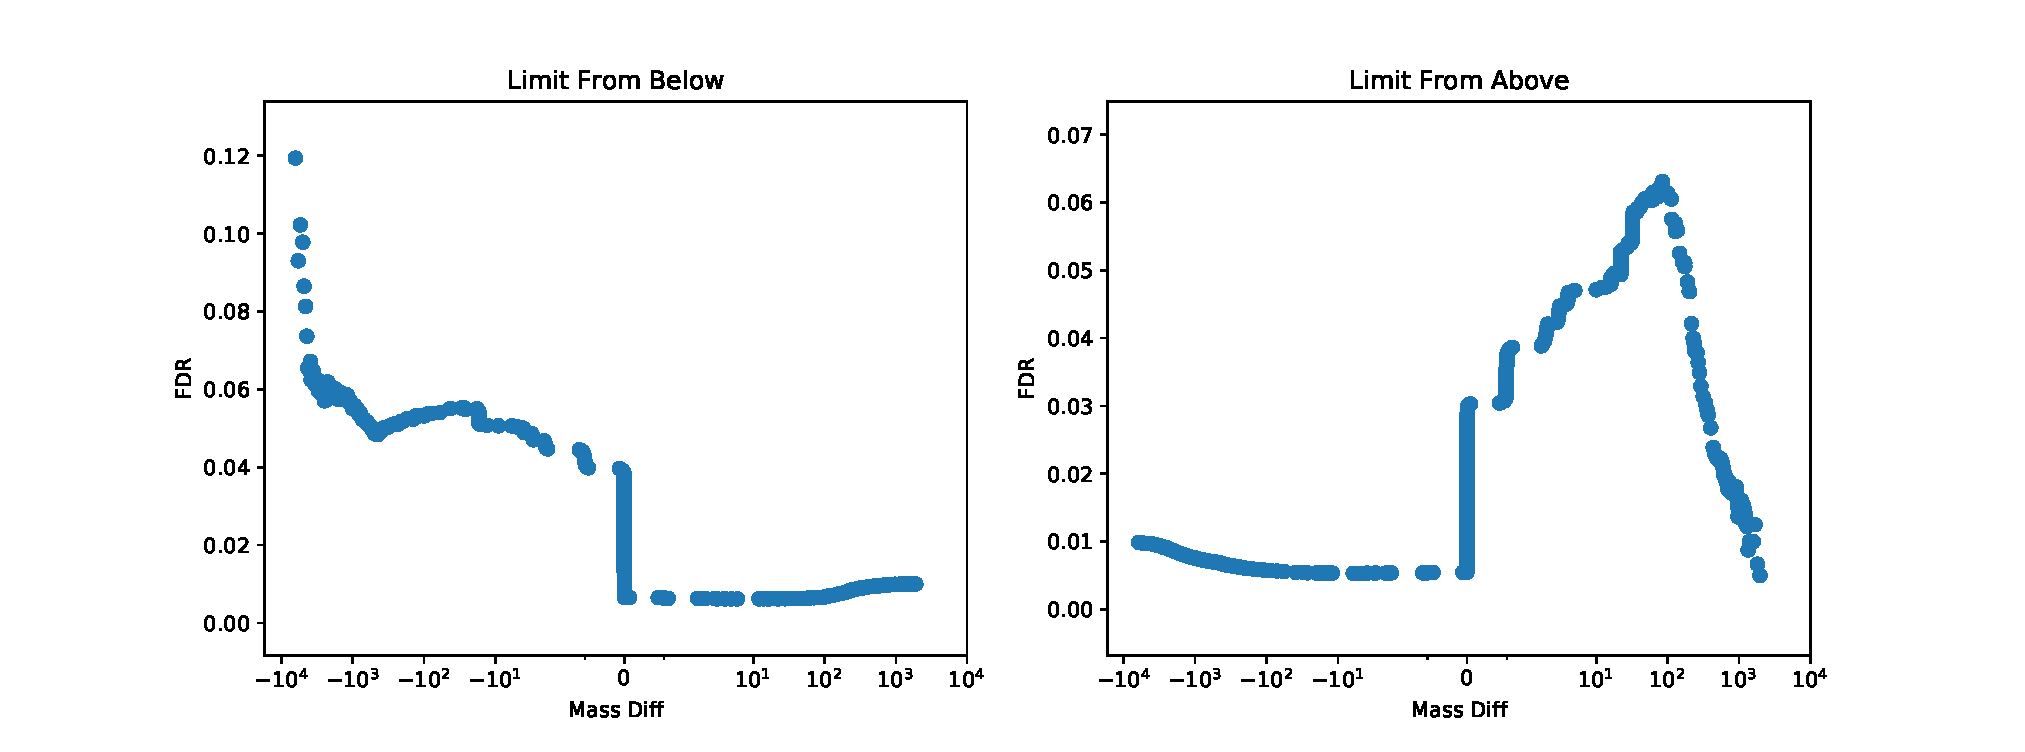
\includegraphics[scale=0.5]{figure_2-upperlowerbounds}
\end{figure}

MetaMorpheus includes a capability to identify peaks in a mass shift histogram obtained from a search, using a recently described peak finding algorithm\cite{Rodriguez_2014}.
We identified peaks with anomalously high false discovery rates, which could be excluded from wide mass searches in order to improve the overall identification quality.
Some histogram peaks are illustrated in Figure~\ref{fig:figure3}, including peaks corresponding to masses of Sulfo and Phospho, and a problematic peak at mass of Leucine, with a high FDR.

\begin{figure}
\caption{Some Histogram Peaks For Mouse Data}
\label{fig:figure3}
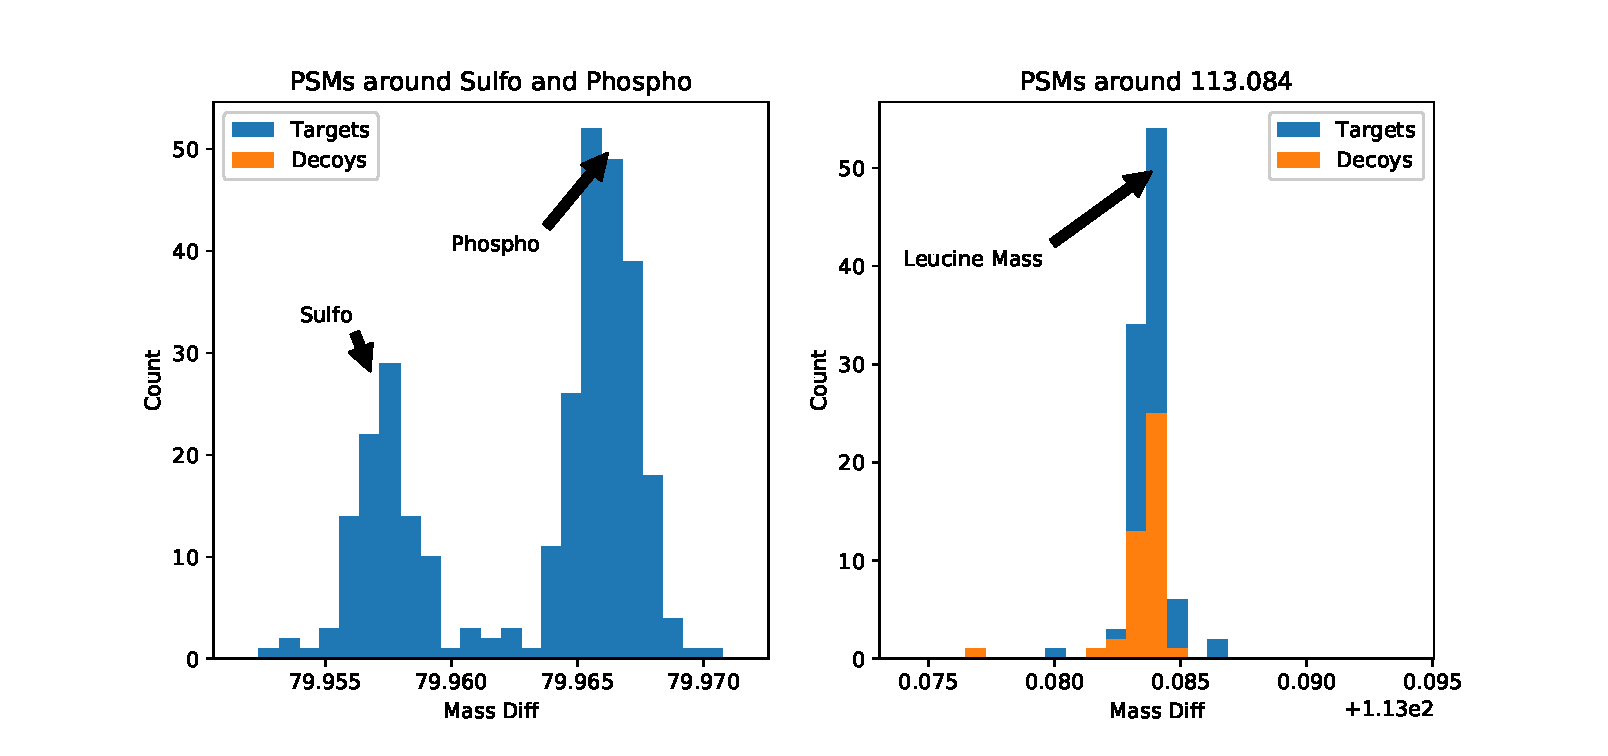
\includegraphics[scale=0.6]{figure_3peaks}
\end{figure}

We identified the property of some specific mass shifts that correspond to anomalously high false discovery rates: these mass shifts correspond precisely to various combinations of residue mass additions and removals.

Mass windows provide an mechanism to exclude these problematic mass shifts from a wide-mass search by employing a interval search.

\subsection{Enhanced G-PTM-D}

By employing the novel notch search strategy instead of the wide-mass search in the G-PTM-D process, using only the modifications listed in Uniprot, the number of confidently identified PSMs increased by 6\%.
The overall search time dropped significantly, from 35 hours to 4 hours for all datasets, see Table~\ref{my-label}.

\begin{table}[]
\centering
\caption{Effects of Replacing Initial Wide-Mass Search by a Notch Search}
\label{my-label}
\begin{tabular}{ll|l|l}
                      &        & Wide-Mass Search & Notch Search\\
\hline
\multirow{2}{*}{Time} & Jurkat & 22.1 hrs         & 2.9 hrs    \\
                      & Mouse  & 13.5 hrs         & 1.2 hrs   \\
\hline
\multirow{2}{*}{PSMs} & Jurkat & 203237           & 210566    \\
                      & Mouse  & 153674           & 162473   
\end{tabular}
\end{table}


The final search with the augmented database is conducted with notches: we only recommend including the common missed monoisotopic mass values in the final search,.
The effect of using these notches is shown in Table~\ref{tab:table2}.

\begin{table}[]
\centering
\caption{Effects of Replacing Final Narrow-Mass Search by a Notch Search}
\label{tab:table2}
\begin{tabular}{ll|l|l}
                      &        & Narrow-Mass Search & Notch Search\\
\hline
\multirow{2}{*}{PSMs} & Jurkat  & 210566   &  220574  \\
                      & Mouse    & 162473   &   170743
\end{tabular}
\end{table}

Since the XML database is annotated with PTMs from the UniProt PTM list, it is natural to use it in the augmentation step as well.
It has a few significant drawbacks: Some mass values do not correspond to actual mass shifts, lability of modifications is not taken into account, and many PTMs are missing, including adducts and glycosylations.
Notch searches allow using expanded modification lists that include chemical modifications such as adducts and large mass PTMs such as glycosylations.
Even though adducts arising from experimental artifacts are not ultimately interesting to biologists, not including them as an option decreases the total number of identified proteins and PTMS.
A curated set of notches and the corresponding modifications is given in Appendix A.
The overall identification rate increased from 164,697 to 179,345 peptide-spectral matches (PSMs), which in turn increased the number of modified peptides by an additional 20\%.
We identified hundreds of glycosylated peptides in these unenriched samples, with many of these modifications exceeding 1000 Daltons. 

\begin{table}[]
\centering
\caption{Effects of Using Different Modification Lists}
\label{tab:table3}
\begin{tabular}{ll|l|l|l}
                      &        & Only Uniprot & Uniprot+Glyco & Uniprot+Glyco+Adducts\\
\hline
\multirow{2}{*}{PSMs} & Jurkat  & 220574   &  222985 & 223578\\
                      & Mouse    & 170743   &   171432& 174783 
\end{tabular}
\end{table}

The initial notch search is significantly faster than a corresponding wide mass search, and this suggests that multiple search rounds could be conducted, iteratively adding more and more modifications.
This recursive nature of the algorithm is well suited to add multiple modifications of different types on the same peptide.
Due to these enhancements, we test the performance of our methods 

\begin{table}[]
\centering
\caption{My caption}
\label{my-label}
\begin{tabular}{|l|l|l|l|l|l|}
\hline
                      &        & \multicolumn{2}{l|}{Single Round}                                                                              & \multicolumn{2}{l|}{Multiple Rounds}                                                                           \\ \hline
                      &        & \begin{tabular}[c]{@{}l@{}}Mods:\\ none\end{tabular} & \begin{tabular}[c]{@{}l@{}}Mods:\\ ptmlist\end{tabular} & \begin{tabular}[c]{@{}l@{}}Mods:\\ none\end{tabular} & \begin{tabular}[c]{@{}l@{}}Mods:\\ ptmlist\end{tabular} \\ \hline
\multirow{2}{*}{PSMs} & Jurkat &                                                      &                                                         &                                                      &                                                         \\ \cline{2-6} 
                      & Mouse  &                                                      &                                                         &                                                      &                                                         \\ \hline
\multirow{2}{*}{Mods} & Jurkat &                                                      &                                                         &                                                      &                                                         \\ \cline{2-6} 
                      & Mouse  &                                                      &                                                         &                                                      &                                                         \\ \hline
\multirow{2}{*}{Time} & Jurkat &                                                      &                                                         &                                                      &                                                         \\ \cline{2-6} 
                      & Mouse  &                                                      &                                                         &                                                      &                                                         \\ \hline
\end{tabular}
\end{table}


\subsection{Discovery of Modifications not in Database}

Previously described wide mass search strategies for discovery and localization of unknown modifications benefit from using alternative, carefully designed search modes based on interval and notch searches.
We discovered that limiting mass shifts to a lower bound of -187 Da (corresponding to the largest mass difference that could be attributed to loss of a single residue, Tryptophan), and no upper bound, is an important step in eliminating spurious PSMs.
Furthermore, treating highly suspect mass shifts corresponding to residue additions/substitutions/deletions in a separate notch search with individualized false discovery rate estimates is beneficial.
An automated tool built into MetaMorpheus allows confidently identifying novel modifications based on these search results.


%
\begin{acknowledgement}

The authors thank \ldots
\end{acknowledgement}

\begin{suppinfo}

The following files are available free of charge.
\begin{itemize}
  \item Filename: brief description
  \item Filename: brief description
\end{itemize}

\end{suppinfo}

\newpage

\bibliography{citations}

\end{document}
